\documentclass[hidelinks]{article}
\usepackage[a4paper, total={7in, 10in}]{geometry}
\usepackage[dvipsnames]{xcolor}
\usepackage{amsmath, amssymb}
\usepackage{amsfonts}
\usepackage{tikz}
\usepackage{tkz-euclide}
\usepackage[unicode]{hyperref}
\usepackage[all]{hypcap}
\usepackage{fancyhdr}
\usepackage{hyperref}
\usepackage{booktabs} % For better table formatting
\usepackage{siunitx}  % For scientific notation formatting

\usetikzlibrary{angles,calc, decorations.pathreplacing}

\definecolor{carminered}{rgb}{1.0, 0.0, 0.22}
\definecolor{capri}{rgb}{0.0, 0.75, 1.0}
\definecolor{brightlavender}{rgb}{0.75, 0.58, 0.89}

\title{\textbf{MATH598B Homework 1}}
\author{Alex Fruge}
\date{February 11, 2025}
\begin{document}
	\hypersetup{bookmarksnumbered=true,}
	\maketitle

	
	\begin{Large}
			Suppose we have a vector space $\mathbb{R}^d$, with $n$ vectors in this space. 
	\end{Large}
	
	\section{Question 1}

	\textit{What is the maximum number $n$ of orthogonal vectors we can put into this vector space? Explain why, in detail.}\\
	
	{\color{Thistle}{\textbf{Answer:} the maximum number of orthogonal vectors that can fit into $\mathbb{R}^d$ is $d$.}}
	
	\textbf{Why?:}
		
	For two vectors to be orthogonal, their inner product must be zero. In order for a group of vectors to be orthogonal, this relation must hold true for all pairs of vectors within the group. One useful property we get when assuming that the vectors are orthogonal is that they are also linearly independent, which helps us set the upper bound for the number of vectors in the vector space.
	
	Since $\mathbb{R}^d$ is a $d$-dimensional space, the maximum number of linearly independent vectors in $\mathbb{R}^d$ is $d$. Since orthogonal vectors are also linearly independent, it also follows that the maximum number of orthogonal vectors in $\mathbb{R}^d$ is $d$.
	
	An example of this is the standard basis vectors for $\mathbb{R}^d$. 
	
	\[e_1 = (1,0,0,\dots,0),\quad e_2 = (0,1,0,\dots,0),\quad\dots,\quad e_d = (0,0,0,\dots,1)\]
	
	These vectors satisfy $e_i \cdot e_j = 0$ for $i\ne j$, which means that there are $d$ orthogonal vectors in $\mathbb{R}^d$.
	
	\section{Question 2}
	
	\textit{Suppose we concatenate the $n$ orthogonal vectors, each in $\mathbb{R}^d$, into a single matrix. What properties will this matrix have? Be thorough.}
	
	{\color{Thistle}{\textbf{Answer:}}} Let the matrix $A$ be defined by concatenating $n$ orthogonal vectors in $\mathbb{R}^d$. If the vectors are normalized, then they form an \textbf{orthonormal} set $(v_i ^\intercal v_j = 0 \text{ for } i \ne j, v_i ^\intercal v_i = 1)$. If this is the case, then we can say that $A$ is \textbf{semi-orthogonal}, which means that $A ^\intercal A = I_n$ where $I_n$ is the $n\times n$ identity matrix. 
	
	Since the columns are orthogonal and non-zero, they are \textbf{linearly independent}, which means that \textbf{$\text{rank } A = \text{min}(n,d)$} If $n \le d$ .
	
	(\textit{Note:} if $n = d$, and the columns are orthonormal, then $A$ is orthogonal)
	

	
	\section{Question 3}
	
	\textit{Suppose $n\gg d$. Assuming they are packed "optimally", what bounds can we place on the expected dot product of two random vectors from our set? To answer this, you should do some mix of reading papers, trying to derive a bound, and doing numerical experiments. Include your code, cite your sources.}\\
	
	In this context, for the vectors to be packed optimally, I'll be assuming that they are uniformly distributed in the unit sphere in $\mathbb{R}^d$. In this situation, we can take two independently sampled vectors from our space, and find the expected value of their dot product.
	
	I'll be using a simulation (\url{https://github.com/alexfruge/decoding-gpt-fruge/blob/main/Homework/hw1sim.py}) to gain some initial intuition as to what these bounds could be.
	\\
	
	\begin{table}[h!]
		\centering
		\begin{tabular}{c S[table-format=1.6e-2] S[table-format=1.6e-2]}
			\toprule
			\textbf{Dimension (\(d\))} & \textbf{Mean Dot Product} & \textbf{Variance} \\
			\midrule
			10    & 5.320471e-05   & 2.040759e-07  \\
			50    & 2.963093e-05   & 3.253653e-08  \\
			100   & 2.457548e-05   & 1.105645e-08  \\
			500   & 7.106165e-06   & 5.118772e-09   \\
			1000  & 7.432451e-06   & 1.155743e-09  \\
			\bottomrule
		\end{tabular}
		\caption{Mean Dot Product and Variance for Different Dimensions}
		\label{tab:dot_product_stats}
	\end{table}
	
	\begin{figure}[h]
		\centering
		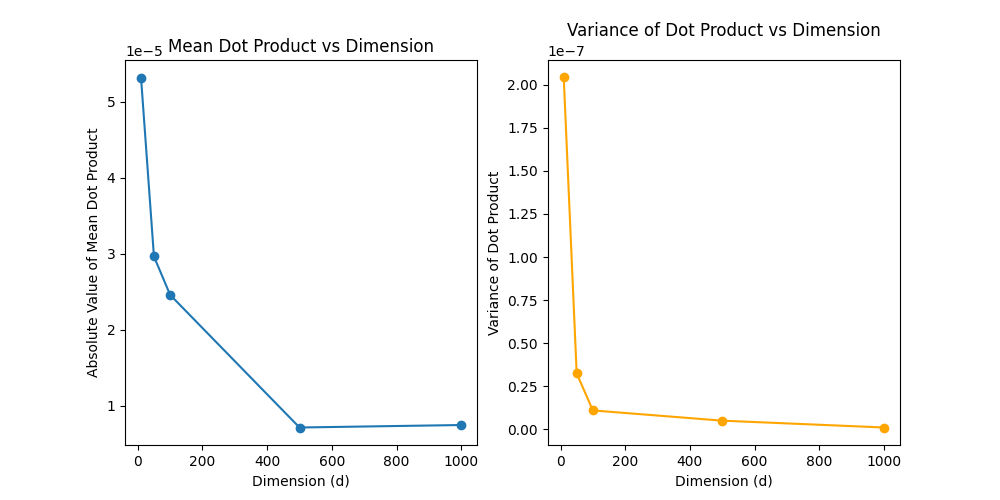
\includegraphics[width=6in]{simfig.png}
		\caption{Plot showing simulation results for mean dot product and variance of dot products as dimension changes.}
	\end{figure}
	
	It appears that as dimension increases, the expected dot product of two vectors approaches zero, as well as the variance of the dot product. The expected values approach zero as the dimension increases, showing that the larger $d$ gets, the closer our vectors get to truly being orthogonal. The relationship variance has with dimension is also reasonable, as one could expect that as more dimensions are added, there are more chances for the vector to reach orthogonality, meaning that the deviations from orthogonality are smaller, leading to a smaller variance.
	
	\section{Question 4}
	\textit{Why do you think thinking about this is relevant for the subject of the course? What do you think these vectors are supposed to represent, and why might we care about them being "optimally packed"?}
	
	The vectors likely represent the embeddings that we feed whatever network we're training at the time. The reason we care about them being optimally packed is that by spacing out the vectors as much as possible, we are able to minimize errors, and maximize error detection.
	\newpage
	
	\section{LLM Logs}
	
	\textit{Here's a prompt that I asked for question 3: } Suppose we have a vector space $\mathbb{R}^d$, with $n$ vectors in this space. Assume that $n \gg d$. What kind of bounds could be useful for finding the expected value of two random vectors from the set?
	
	\textit{ChatGPT-4o Response: }Given $n$ vectors in $\mathbb{R}^d$ with $n \gg d$, a useful approach for finding the expected value of the dot product (or other function) of two randomly chosen vectors is to consider concentration inequalities and properties of high-dimensional geometry. Here are some useful tools and bounds:\\
	
	\textbf{Concentration of Measure}: In high-dimensional spaces, random vectors tend to be nearly orthogonal. Specifically, if the vectors are normalized, the dot product between two randomly chosen vectors is close to zero with high probability. This can be formalized using concentration inequalities like Hoeffding's inequality or McDiarmid's inequality, depending on the dependence structure.\\
	
	\textbf{Johnson-Lindenstrauss Lemma}: This lemma states that a set of $n$ points in $\mathbb{R}^d$	can be embedded into $\mathbb{R}^k$ (with $k = O(\log n / \epsilon^2)$) such that pairwise distances are approximately preserved. This can be used to bound the expected distance or dot product between two vectors, as the reduced dimensionality preserves the geometric structure.\\
	
	\textbf{Inner Product Expectation}: If the vectors are drawn uniformly from the unit sphere $S^{d-1}$, then the expected dot product between two randomly chosen vectors is: \[\mathbb{E}[\langle X, Y \rangle] = 0\] because of symmetry. The variance is $\frac{1}{d}$, suggesting that the dot products are typically small when $d$ is large.\\
	
	\textbf{Random Matrix Theory}: If the vectors are organized into a matrix $A$ of size $d \times n$, then properties of the Gram matrix $G = A^{\intercal}A$(e.g., spectral norm bounds) can provide information about the correlations between the vectors.\\
	
	\textbf{Covering Numbers and Metric Entropy}: For understanding the distribution of the vectors, bounds on covering numbers or metric entropy can provide insight into the expected geometric arrangement of the vectors, which can, in turn, help estimate expected values of distances or dot products.\\
	
	If you can provide more specifics about the distribution of the vectors or the exact expected value you're looking for, I can tailor the bounds and tools more precisely!\\

	\textit{Prompt intent: }I intended for this prompt to be a little more general, but 4o went into a good bit of detail, which ended up being useful to kickstart my own research into the problem.
		
\end{document}
